\newpage
\section{Task 2: Advanced normalisation}

Figure 2 below depicts an invoice for an order from a store.

\begin{figure}[H]
\centering
\caption{Pakoko Tax Invoice}
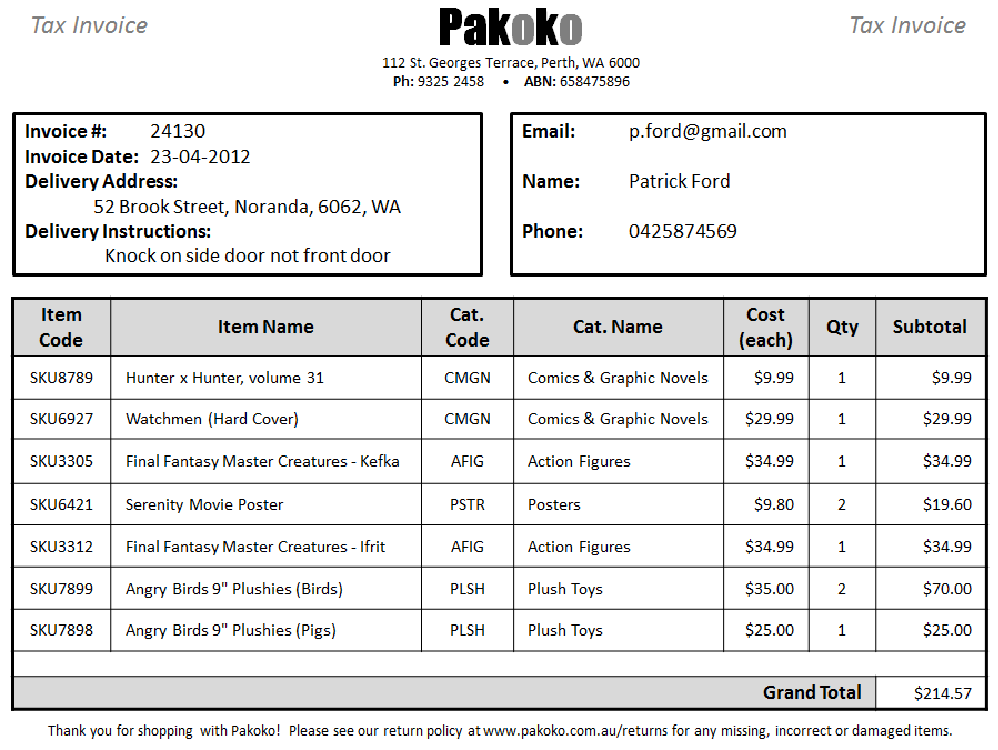
\includegraphics[scale=0.75]{./img/task2.pdf}
\end{figure}

\subsection{Assumptions}

\begin{itemize}
\item Auto-incrementing Cust\# has been created, replacing CustEmail as customer identifier
	\begin{itemize}
	\item Auto-incrementing identifier avoids user input error which may result in multiple customers with the same email address
	\item Allows CustEmail to be updated without having to update foreign keys if CustEmail remained as identifier
	\end{itemize}
\item Each item is only in one category
\item Item codes are unique per item, even if the items are in different categories
\item Invoice header and footer is static and is not stored in the database
	\begin{itemize}
	\item Includes Pakoko business details header and thank you / return policy URL footer
	\end{itemize}
\item Derived attributes are not stored in the database
	\begin{itemize}
	\item Includes Item Subtotal and Invoice Grand Total
	\end{itemize}
\end{itemize}

\subsection{0NF: Unnormalised form}

R1 = (Cust\#, CustEmail, CustName, CustPhone, DeliveryAddress, DeliveryInstructions, \{Invoice\#, InvoiceDate, \{ItemCode, ItemName, CatCode, CatName, Cost, Qty\}\})

\subsection{1NF: First normal form}

\sout{R1 = (\textbf{\underline{Cust\#}}, CustEmail, CustName, CustPhone, DeliveryAddress, DeliveryInstructions, \{\textbf{\underline{Invoice\#}}, InvoiceDate, \{\textbf{\underline{ItemCode}}, ItemName, CatCode, CatName, Cost, Qty\}\})}
\\\\
R11 = (\textbf{\underline{Cust\#}}, CustEmail, CustName, CustPhone, DeliveryAddress, DeliveryInstructions)
\\\\
R12 = (\textbf{\underline{Invoice\#}}, InvoiceDate, \emph{Cust\#})
\\\\
R13 = (\textbf{\underline{\emph{Invoice\#}}}, \textbf{\underline{ItemCode}}, ItemName, CatCode, CatName, Cost, Qty)

\subsection{2NF: Second normal form}

R11 = (\textbf{\underline{Cust\#}}, CustEmail, CustName, CustPhone, DeliveryAddress, DeliveryInstructions)
\\\\
R12 = (\textbf{\underline{Invoice\#}}, InvoiceDate, \emph{Cust\#})
\\\\
\sout{R13 = (\textbf{\underline{\emph{Invoice\#}}}, \textbf{\underline{ItemCode}}, ItemName, CatCode, CatName, Cost, Qty)}
\\\\
R131 = (\textbf{\underline{\emph{Invoice\#}}}, \textbf{\underline{\emph{ItemCode}}}, Qty)
\\\\
R132 = (\textbf{\underline{ItemCode}}, ItemName, CatCode, CatName, Cost)

\subsection{3NF: Third normal form}

R11 = (\textbf{\underline{Cust\#}}, CustEmail, CustName, CustPhone, DeliveryAddress, DeliveryInstructions)
\\\\
R12 = (\textbf{\underline{Invoice\#}}, InvoiceDate, \emph{Cust\#})
\\\\
R131 = (\textbf{\underline{\emph{Invoice\#}}}, \textbf{\underline{\emph{ItemCode}}}, Qty)
\\\\
\sout{R132 = (\textbf{\underline{ItemCode}}, ItemName, CatCode, CatName, Cost)}
\\\\
R1321 = (\textbf{\underline{ItemCode}}, ItemName, \emph{CatCode})
\\\\
R1322 = (\textbf{\underline{CatCode}}, CatName)

\subsection{Named relations}

Customer = (\textbf{\underline{Cust\#}}, CustEmail, CustName, CustPhone, DeliveryAddress, DeliveryInstructions)
\\\\
Invoice = (\textbf{\underline{Invoice\#}}, InvoiceDate, \emph{Cust\#})
\\\\
InvoiceItem = (\textbf{\underline{\emph{Invoice\#}}}, \textbf{\underline{\emph{ItemCode}}}, Qty)
\\\\
Item = (\textbf{\underline{ItemCode}}, ItemName, \emph{CatCode})
\\\\
Category = (\textbf{\underline{CatCode}}, CatName)

\subsection{Physical E-R diagram}